

\section{Bayesian Skip-Gram}

\begin{frame}[plain]{Bayesian Skip-Gram}


\begin{columns}
\begin{column}{0.45\textwidth}
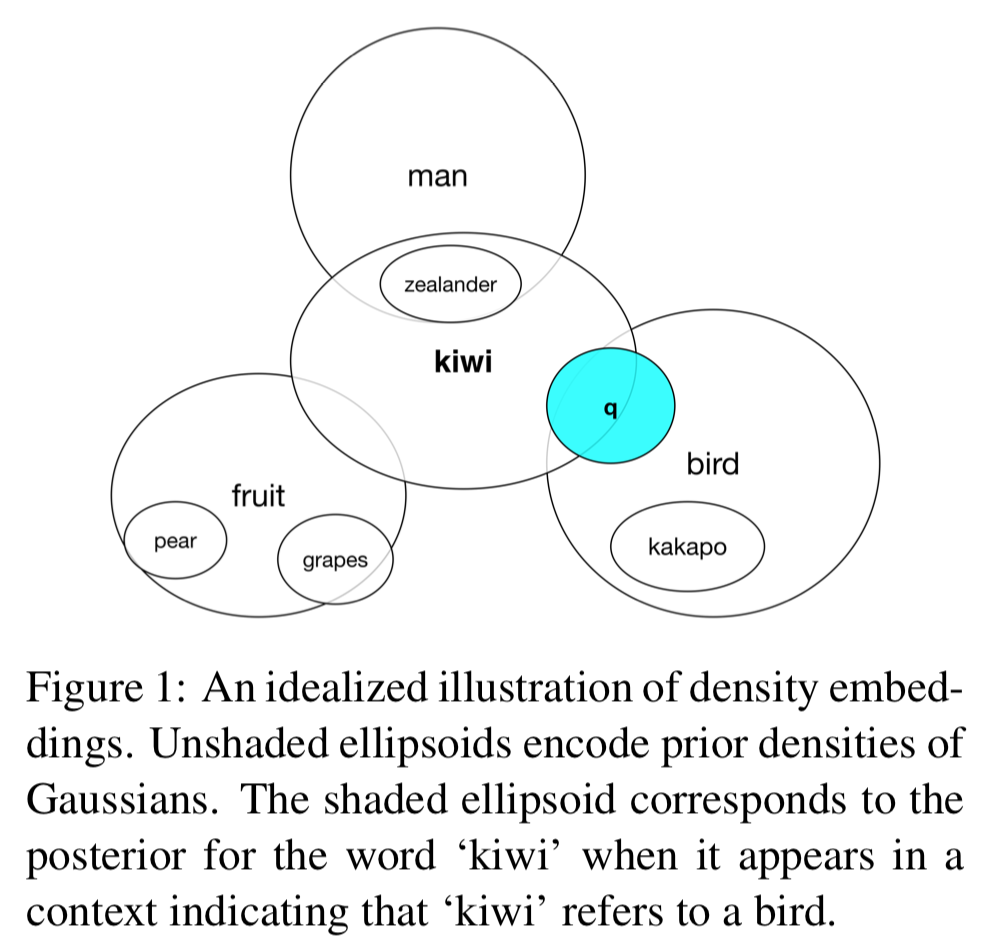
\includegraphics[scale=0.35]{img/bsg-example}
\end{column}
\quad
\begin{column}{0.45\textwidth}
\begin{footnotesize}
\only<1>{
\emph{``Representing a word as a distribution provides many potential benefits. For example, such embeddings let us encode generality of terms (e.g., `kakapo' is a type of `bird'), characterize uncertainty about semantic properties of the corresponding referent (e.g., a proper noun, such as `John', encodes little about the person it refers to) or represent polysemy (e.g., `kiwi' may refer to a fruit, a bird or a New Zealander).''}
}
\only<2>{
\emph{``In principle, using densities to represent words provides a natural way of encoding entailment: the decision regarding entailment relation can be made by testing the level sets of the distributions for `soft inclusion'. For example, in Figure 1, the ellipse for `kakapo' lies within the ellipse for `bird'. ''}
}
\end{footnotesize}
\end{column}

\end{columns}


\ack{\citet{bravzinskas2017embedding}}
\end{frame}


\begin{frame}[plain]{Complete specification}
Generative model: for $i=1, \ldots, m$\\

\begin{equation*}
\begin{aligned}
Z_i|x_i &\sim \mathcal N(\boldsymbol \mu_{x_i}, \diag(\boldsymbol \sigma_{x_i} \odot \boldsymbol \sigma_{x_i}))\\
\boldsymbol \mu_{x_i} &= \text{lookup}_\theta(x_i)\\
\boldsymbol \sigma_{x_i} &= \softplus(\text{lookup}_\theta(x_i))
\end{aligned}
\end{equation*}
\pause
~for $k \in \mathcal K_i = \{\underbrace{i-n, \ldots, i-1,  i+1, \ldots, i+n}_{n \text{ words on each side of }x_i}\}$ \pause
\begin{equation*}
\begin{aligned}
X_k|z_i &\sim \Cat(\mathbf f_i) \\ 
\mathbf f_i &= \softmax(\affine_\theta(z_i))
\end{aligned}
\end{equation*}

\pause

Inference model
\begin{equation*}
\begin{aligned}
Z_i|x_{i-n}^{i+n} &\sim \mathcal N(\mathbf u_i, \diag(\mathbf s_i \odot \mathbf s_i))\\
\mathbf h_i &= \sum_{k \in \mathcal K_i} \relu(\affine_\lambda([x_k, x_i])) \\
\mathbf u_i &= \affine_\lambda(h_i) \\
\mathbf s_i &= \softplus(\affine_\lambda(h_i)) 
\end{aligned}
\end{equation*}


\end{frame}

\begin{frame}{ELBO}
\begin{equation*}
\begin{aligned}
\mathbb E_{q_\lambda(z_1^m|x_1^m)} \left[ \log \alert{\prod_{i=1}^m \prod_{k \in \mathcal K_i} P(x_k|z_i)} \right] - \KL{q_\lambda(z_1^m|x_1^m)}{p_\theta(z_1^m|x_1^m)}
\end{aligned}
\end{equation*}
\begin{itemize}
	\item observation model is trained discriminatively\\
	latent variables generate overlapping subsets of observations
\end{itemize}

\end{frame}

\begin{frame}{ELBO - KL term}
\begin{equation*}
\begin{aligned}
\mathbb E_{q_\lambda(z_1^m|x_1^m)} \left[ \log \prod_{i=1}^m \prod_{k \in \mathcal K_i} P_\theta(x_k|z_i) \right] - \textcolor{blue}{\KL{q_\lambda(z_1^m|x_1^m)}{p_\theta(z_1^m|x_1^m)}}
\end{aligned}
\end{equation*}

KL term
\begin{equation*}
\begin{aligned}
&\textcolor{blue}{\KL{q_\lambda(z_1^m|x_1^m)}{p_\theta(z_1^m|x_1^m)}} \\ \pause
 &=  \sum_{i=1}^m \KL{q_\lambda(z_i|x_{i-n}^{i+n})}{p_\theta(z_i|x_i)} \\ \pause
 &=  \sum_{i=1}^m \KL{\underbrace{\mathcal N(\mathbf u_i, \diag(\mathbf s_i \odot \mathbf s_i))}_{\text{inference model}}}{\underbrace{\mathcal N(\boldsymbol \mu_{x_i}, \diag(\boldsymbol \sigma_{x_i} \odot \boldsymbol \sigma_{x_i}))}_{\text{prior}}} 
\end{aligned}
\end{equation*}

\ack{Empirical Bayes: point estimate prior parameters}

\end{frame}


\begin{frame}{ELBO - Likelihood term}
\begin{equation*}
\begin{aligned}
\textcolor{blue}{\mathbb E_{q_\lambda(z_1^m|x_1^m)} \left[ \log \prod_{i=1}^m \prod_{k \in \mathcal K_i} P_\theta(x_k|z_i) \right]} - \KL{q_\lambda(z_1^m|x_1^m)}{p_\theta(z_1^m|x_1^m)}
\end{aligned}
\end{equation*}
\pause

Likelihood term
\begin{small}
\begin{equation*}
\begin{aligned}
\textcolor{blue}{\mathbb E_{q_\lambda(z_1^m|x_1^m)} \left[ \log \prod_{i=1}^m \prod_{k \in \mathcal K_i} P_\theta(x_k|z_i) \right]}  \pause
 &= \mathbb E_{q_\lambda(z_1^m|x_1^m)} \left[  \sum_{i=1}^m \sum_{k \in \mathcal K_i} \log P_\theta(x_k|z_i) \right] \\ \pause
&= \sum_{i=1}^m \sum_{k \in \mathcal K_i} \mathbb E_{q_\lambda(z_i|x_{i-n}^{i+n})} \left[  \log P_\theta(x_k|z_i) \right] \\ \pause
&= \sum_{i=1}^m \sum_{k \in \mathcal K_i} \mathbb E_{q_\lambda(z_i|x_{i-n}^{i+n})} \left[  \log \Cat(x_k|\mathbf f_i) \right]
\end{aligned}
\end{equation*}
\end{small}

\end{frame}

\begin{frame}{The softmax problem}

To circumvent an expensive softmax, change the likelihood term
\begin{equation*}
P_\theta(x|z) = \frac{u_\theta(z, x)}{\alert{\sum_{x' \in \mathcal X} u_\theta(z, x')}} \qquad \text{with } u_\theta(\cdot, \cdot) > 0
\end{equation*}
\pause
and re-write the likelihood term
\begin{equation*}
\begin{aligned}
\mathbb E_{q_\lambda(z)} \left[  \log P_\theta(x|z) \right] 
 &= \mathbb E_{q_\lambda(z)} \left[  \log u_\theta(z, x) - \log \alert{\sum_{x'\in \mathcal X}u_\theta(z, x')}\right] \\ \pause
 &=\mathbb E_{q_\lambda(z)} \left[  \log u_\theta(z, x) \right] - \mathbb E_{q_\lambda(z)} \left[ \log \alert{\sum_{x'\in \mathcal X}u_\theta(z, x')}\right]
\end{aligned}
\end{equation*}


\end{frame}

\begin{frame}[plain]{Lowerbound on likelihood term}
Then (by design) let
\begin{equation*}
u_\theta(z, x) = \underbrace{P(x)}_{\text{fixed}}\mathcal N(z|\boldsymbol \mu_x, \diag(\boldsymbol \sigma_x \odot \boldsymbol \sigma_x))
\end{equation*}
\pause

And bound $ \mathbb E_{q_\lambda(z)} \left[ \log \alert{\sum_{x'\in \mathcal X}u_\theta(z, x')}\right] $ \pause
\begin{equation*}
\begin{aligned} 
&=\mathbb E_{q_\lambda(z)} \left[ \log \alert{\sum_{x'\in \mathcal X} P(x)\mathcal N(z|\boldsymbol \mu_x, \diag(\boldsymbol \sigma_x \odot \boldsymbol \sigma_x))} \right] \\ \pause
&=\mathbb E_{q_\lambda(z)} \left[ \log \alert{\mathbb E_{P(x)}\left[ \mathcal N(z|\boldsymbol \mu_x, \diag(\boldsymbol \sigma_x \odot \boldsymbol \sigma_x)) \right]} \right] \\ \pause
&\overset{\text{JI}}{\ge} \mathbb E_{q_\lambda(z)} \left[ \textcolor{blue}{\mathbb E_{P(x)}\left[ \log \mathcal N(z|\boldsymbol \mu_x, \diag(\boldsymbol \sigma_x \odot \boldsymbol \sigma_x)) \right]} \right]
\end{aligned}
\end{equation*}
\pause

\begin{itemize}
	\item $P(x)$ does not depend on $\theta$, we can compute an MC estimate\\
	e.g. empirical (unigram) distribution
\end{itemize}

\end{frame}



